%!TEX program = lualatex
% Arquivo: Template_Estat_Texto.tex

\documentclass[a4paper,12pt]{article}

% =========================================================
% Idioma e tipografia (LuaLaTeX)
% =========================================================
\usepackage[brazilian]{babel}
\usepackage{fontspec}
\setmainfont{Latin Modern Roman}

% =========================================================
% Layout
% =========================================================
\usepackage[top=3cm,bottom=2.5cm,left=3cm,right=2.5cm]{geometry}
\usepackage{setspace}
\onehalfspacing
\usepackage{indentfirst}
\setlength{\parindent}{1.25cm}

% =========================================================
% Matemática (align*, etc.)
% =========================================================
\usepackage{amsmath}
\usepackage{amssymb}

% =========================================================
% Tabelas, listas, figuras
% =========================================================
\usepackage{booktabs}
\usepackage{array}
\usepackage{enumitem}
\setlist[itemize]{noitemsep,topsep=3pt}
\setlist[enumerate]{noitemsep,topsep=3pt}

\usepackage{graphicx}
\usepackage{float}
\usepackage{pdflscape}
\graphicspath{{./}{./imagens/}{./figuras/}}
\usepackage{pdfpages}

% =========================================================
% Links
% =========================================================
\usepackage{hyperref}
\usepackage{xurl}

% =========================================================
% Referências bibliográficas (ABNT)
% =========================================================
\usepackage{csquotes}
\usepackage[
  backend=biber,
  style=abnt
]{biblatex}
\addbibresource{referencias.bib}

\hypersetup{
  colorlinks=true,
  linkcolor=black,
  urlcolor=blue,
  citecolor=black,
  pdfauthor={Israel Oliveira Carneiro; Davi de Sá; José Mauro Elsas},
  pdftitle={Experimento 2 — Lei de Ohm}
}
\usepackage{siunitx}
\usepackage{multirow}

\sisetup{
  output-decimal-marker = {,}
}

% =========================================================
% Dados da capa
% =========================================================
\newcommand{\Instituicao}{Universidade do Estado do Rio de Janeiro}
\newcommand{\Curso}{Física VI -- Oceanografia}
\newcommand{\Professor}{Professor: Alexandre Magno}
\newcommand{\Aluno}{Aluno: Israel Oliveira Carneiro\\ Davi de Sá\\ José Mauro Elsas}
\newcommand{\Cidade}{Rio de Janeiro}
\newcommand{\Ano}{2026}

\title{\textbf{Experimento 2 — Lei de Ohm}}
\author{\Aluno}
\date{\Cidade --- \Ano}

\begin{document}

% =========================================================
% Capa (página de rosto)
% =========================================================
\begin{titlepage}
\centering
{\large \Instituicao \par}
\vspace{0.5cm}
{\large \Curso \par}
\vspace{1.0cm}

{\LARGE \textbf{Experimento 2} \par}
\vspace{0.6cm}
{\Large Lei de Ohm \par}

\begin{figure}[H]
  \centering
  \includegraphics[width=.3\linewidth]{./uerj.jpg}
\end{figure}

\vfill



\begin{flushright}
\Aluno\\
\Professor
\end{flushright}

\vspace{1.0cm}
{\Cidade --- \Ano \par}
\end{titlepage}


\section{Objetivo}

Os objetivos da prática são calcular a média e o desvio padrão da tensão e da corrente elétrica para cada posição do seletor da fonte de alimentação, construir o gráfico da tensão em função da corrente utilizando os valores médios e determinar graficamente a resistência elétrica do resistor.

\section{Introdução}

O estudo da eletricidade desenvolveu-se de forma significativa entre o final do século XVIII e o início do século XIX, especialmente após a apresentação da pilha elétrica por Alessandro Volta, em 1800 \parencite{volta1800}. A disponibilidade de uma fonte relativamente contínua de corrente elétrica permitiu a realização de experimentos mais sistemáticos sobre o comportamento dos circuitos e dos materiais condutores.

Nesse contexto, o físico e matemático alemão Georg Simon Ohm (1789--1854) investigou experimentalmente a relação entre a diferença de potencial aplicada a um condutor e a corrente elétrica que o atravessa \parencite{mactutor_ohm}. Os resultados de seus estudos foram publicados em 1827, na obra \textit{Die galvanische Kette, mathematisch bearbeitet}, cujo título pode ser traduzido como ``O circuito galvânico tratado matematicamente'' \parencite{ohm1827}. Embora suas conclusões tenham recebido pouca atenção inicialmente, os trabalhos de Ohm tornaram-se fundamentais para o desenvolvimento da teoria dos circuitos elétricos \parencite{mactutor_ohm}.

A Primeira Lei de Ohm estabelece que, para determinados materiais e sob condições físicas constantes, especialmente de temperatura, a corrente elétrica que atravessa um condutor é diretamente proporcional à diferença de potencial aplicada entre suas extremidades. Essa relação pode ser representada por

\begin{equation}
V = R I,
\label{eq:primeira_lei_ohm}
\end{equation}

em que $V$ representa a diferença de potencial elétrico, medida em volts (\si{\volt}); $I$ representa a intensidade da corrente elétrica, medida em ampères (\si{\ampere}); e $R$ corresponde à resistência elétrica do condutor, medida em ohms (\si{\ohm}) \parencite[seção 9.4]{ling2016}.

Para um condutor que obedece à Primeira Lei de Ohm, denominado condutor ôhmico, a resistência elétrica permanece aproximadamente constante. Dessa forma, o gráfico da diferença de potencial em função da corrente elétrica apresenta comportamento linear, e o coeficiente angular da reta corresponde ao valor da resistência do componente. Entretanto, materiais ou dispositivos que não apresentam essa proporcionalidade são classificados como não ôhmicos \parencite[seção 9.4]{ling2016}.

A verificação experimental da Primeira Lei de Ohm permite analisar o comportamento elétrico de um resistor, determinar sua resistência a partir de medidas de tensão e corrente e comparar o valor experimental com o valor nominal indicado pelo fabricante. Além disso, o experimento contribui para a compreensão do funcionamento de circuitos elétricos e das limitações associadas às medições realizadas em laboratório.


\section{Materiais e Métodos}

Foram os seguintes os materiais utilizados para a execução do Experimento:

\begin{enumerate}[label=\alph*.]
    \item Voltímetro analógico com pontas de prova. \par\vspace{0.5\baselineskip}
        \begin{figure}[H]
      \centering
      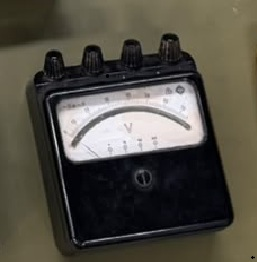
\includegraphics[width=0.4\linewidth]{./Figs/volt.jpg}
    \end{figure}

    \item Miliamperímetro analógico \par\vspace{0.4\baselineskip}
            \begin{figure}[H]
      \centering
      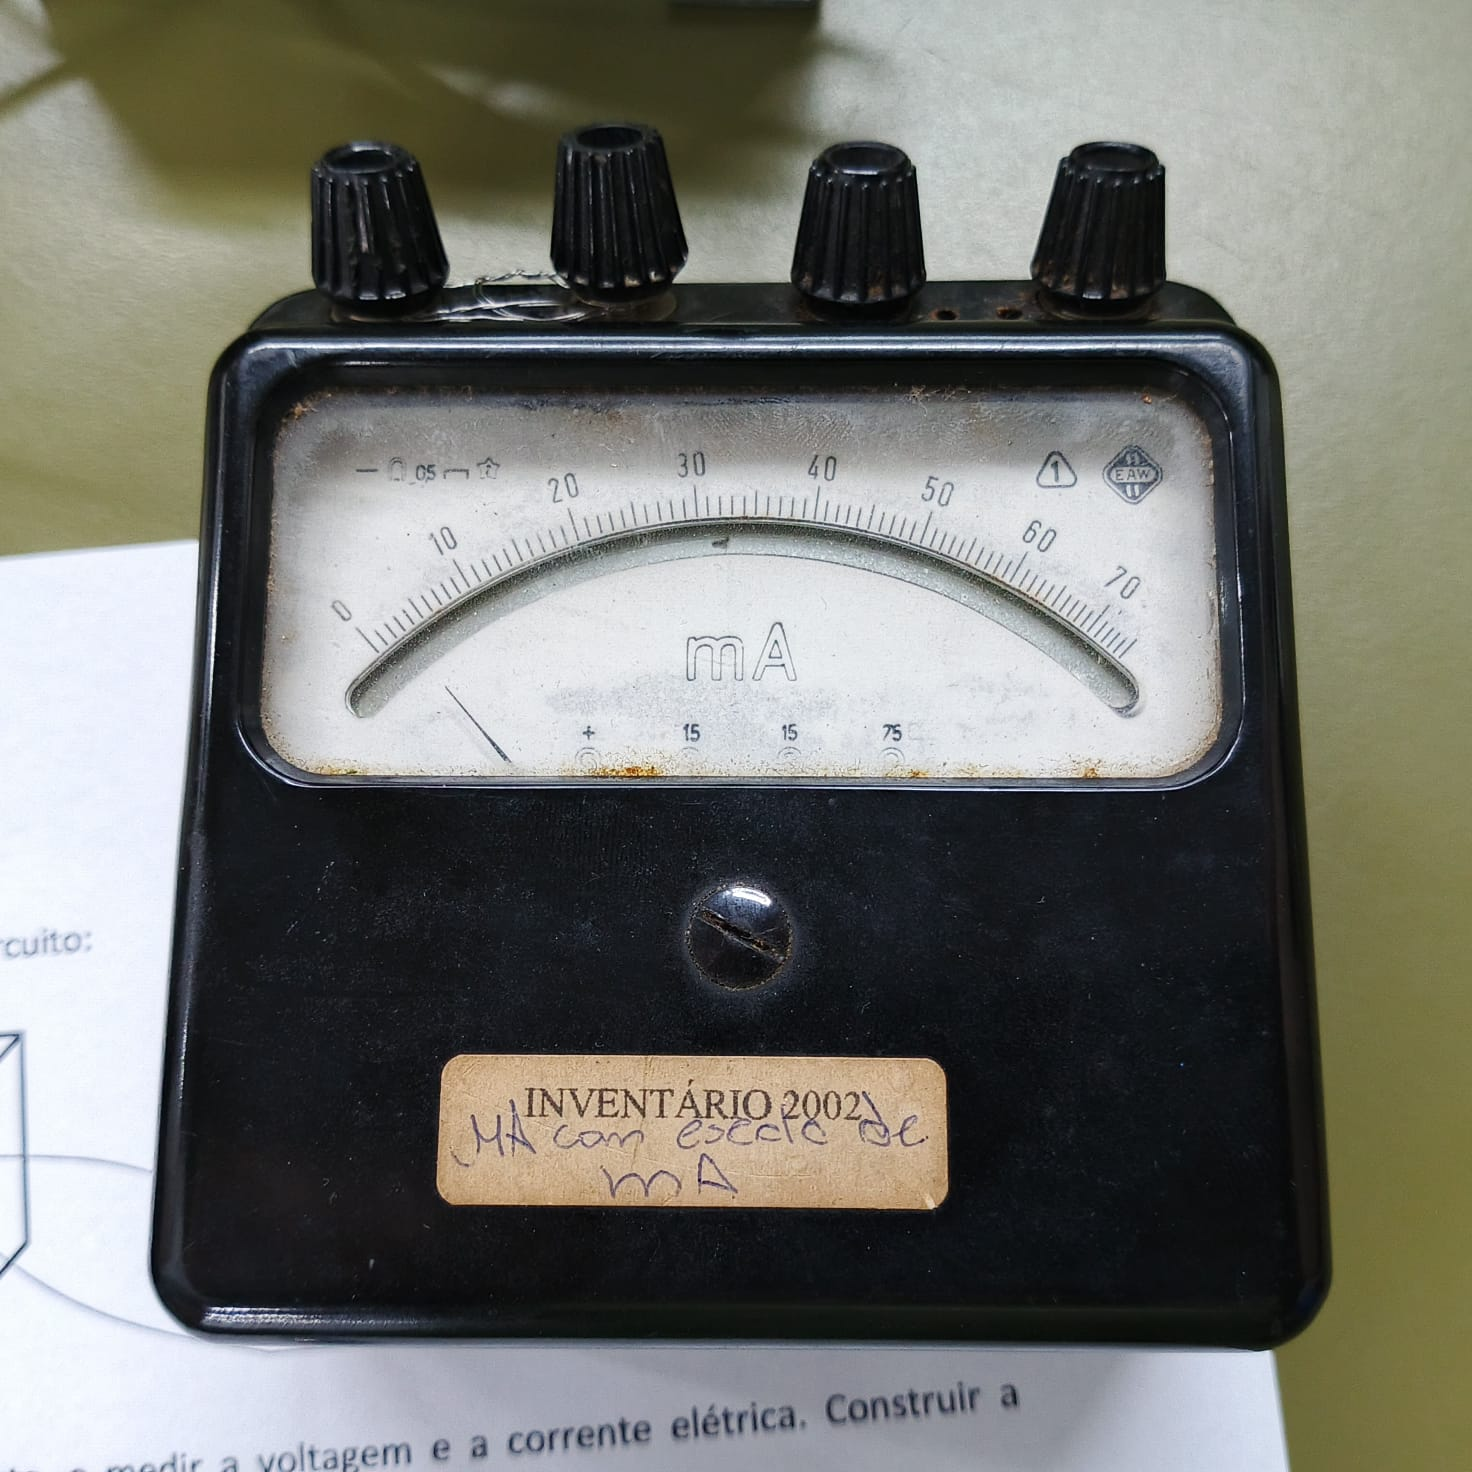
\includegraphics[width=0.4\linewidth]{./Figs/miliamp.jpeg}
    \end{figure}

    \item Fonte de alimentação. \par\vspace{0.5\baselineskip}
        \begin{figure}[H]
      \centering
      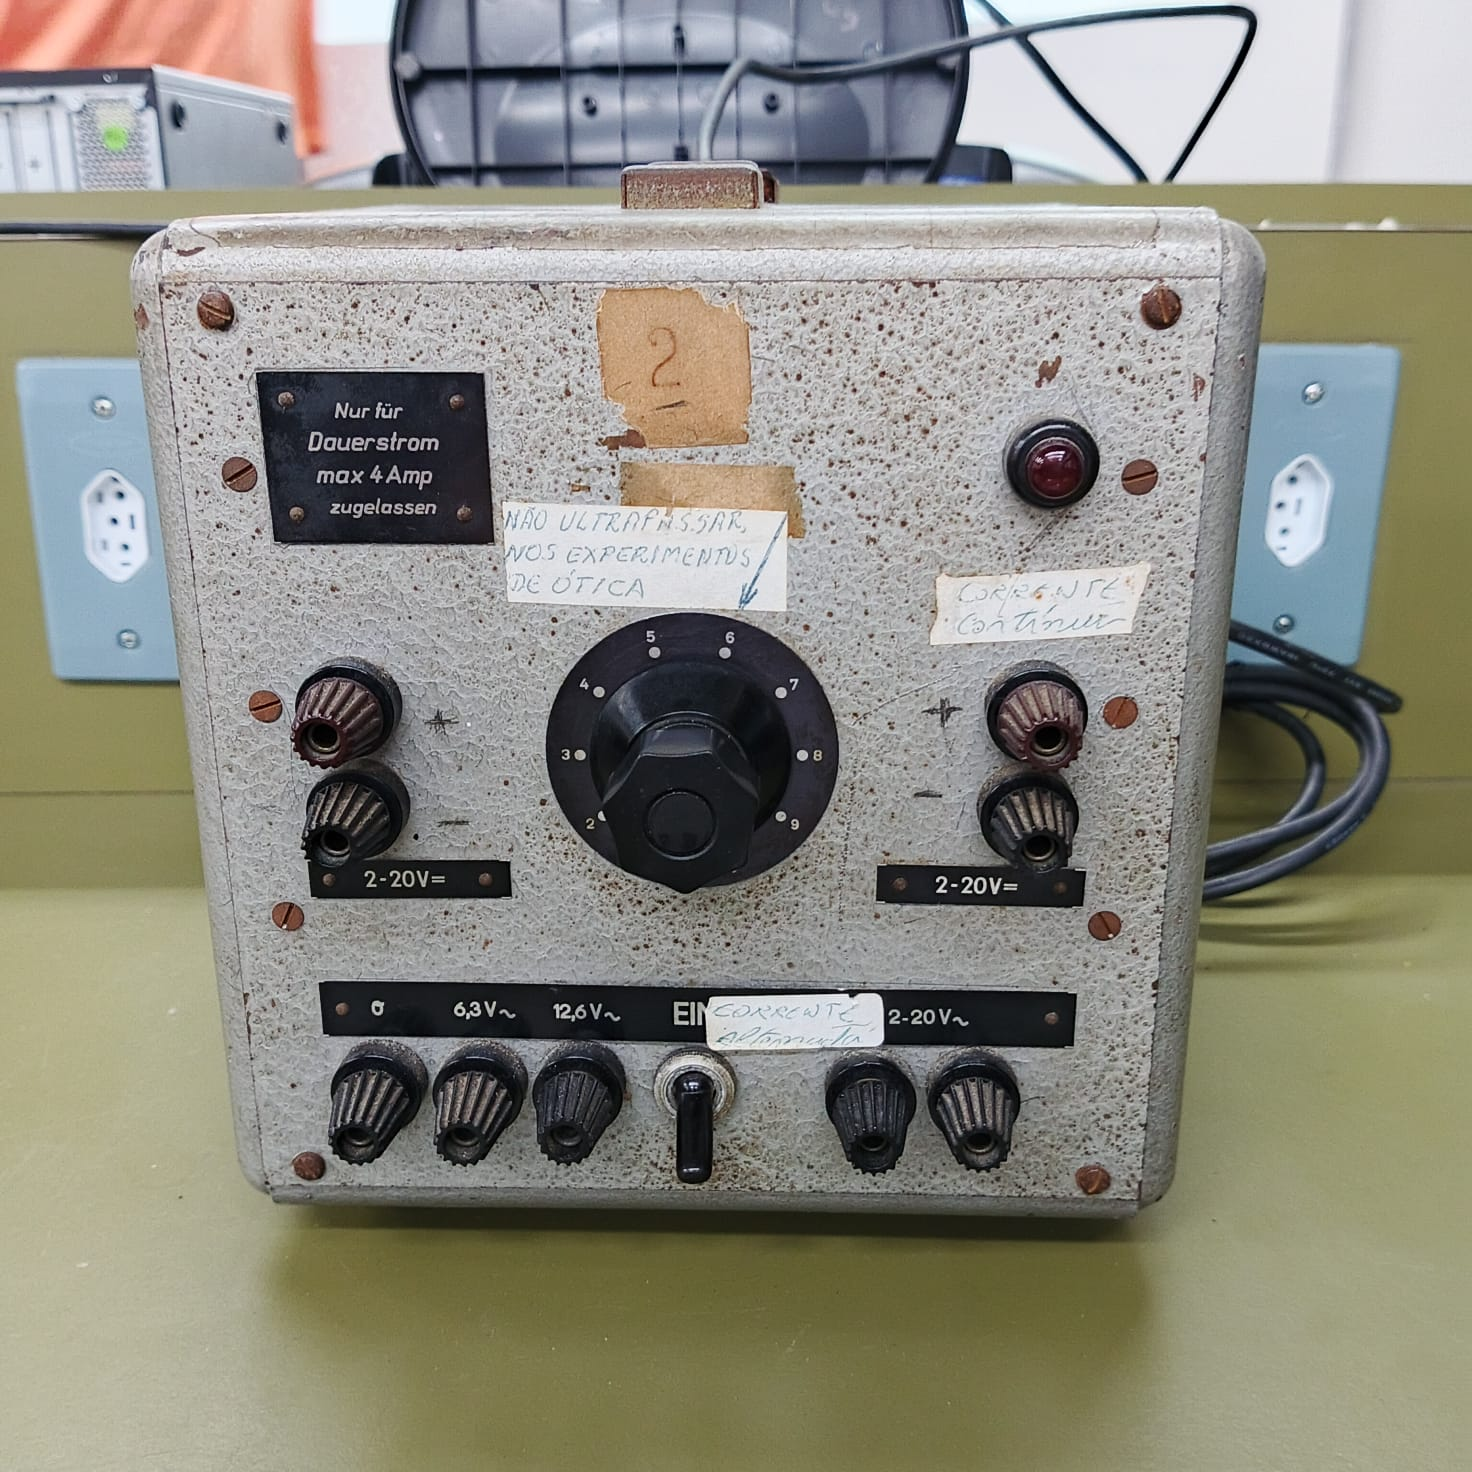
\includegraphics[width=0.4\linewidth]{./Figs/fonte.jpeg}
    \end{figure}
    
    \item Resistor de $\SI{390}{\,\ohm}\,\pm 5\%$. \par\vspace{0.5\baselineskip}
            \begin{figure}[H]
      \centering
      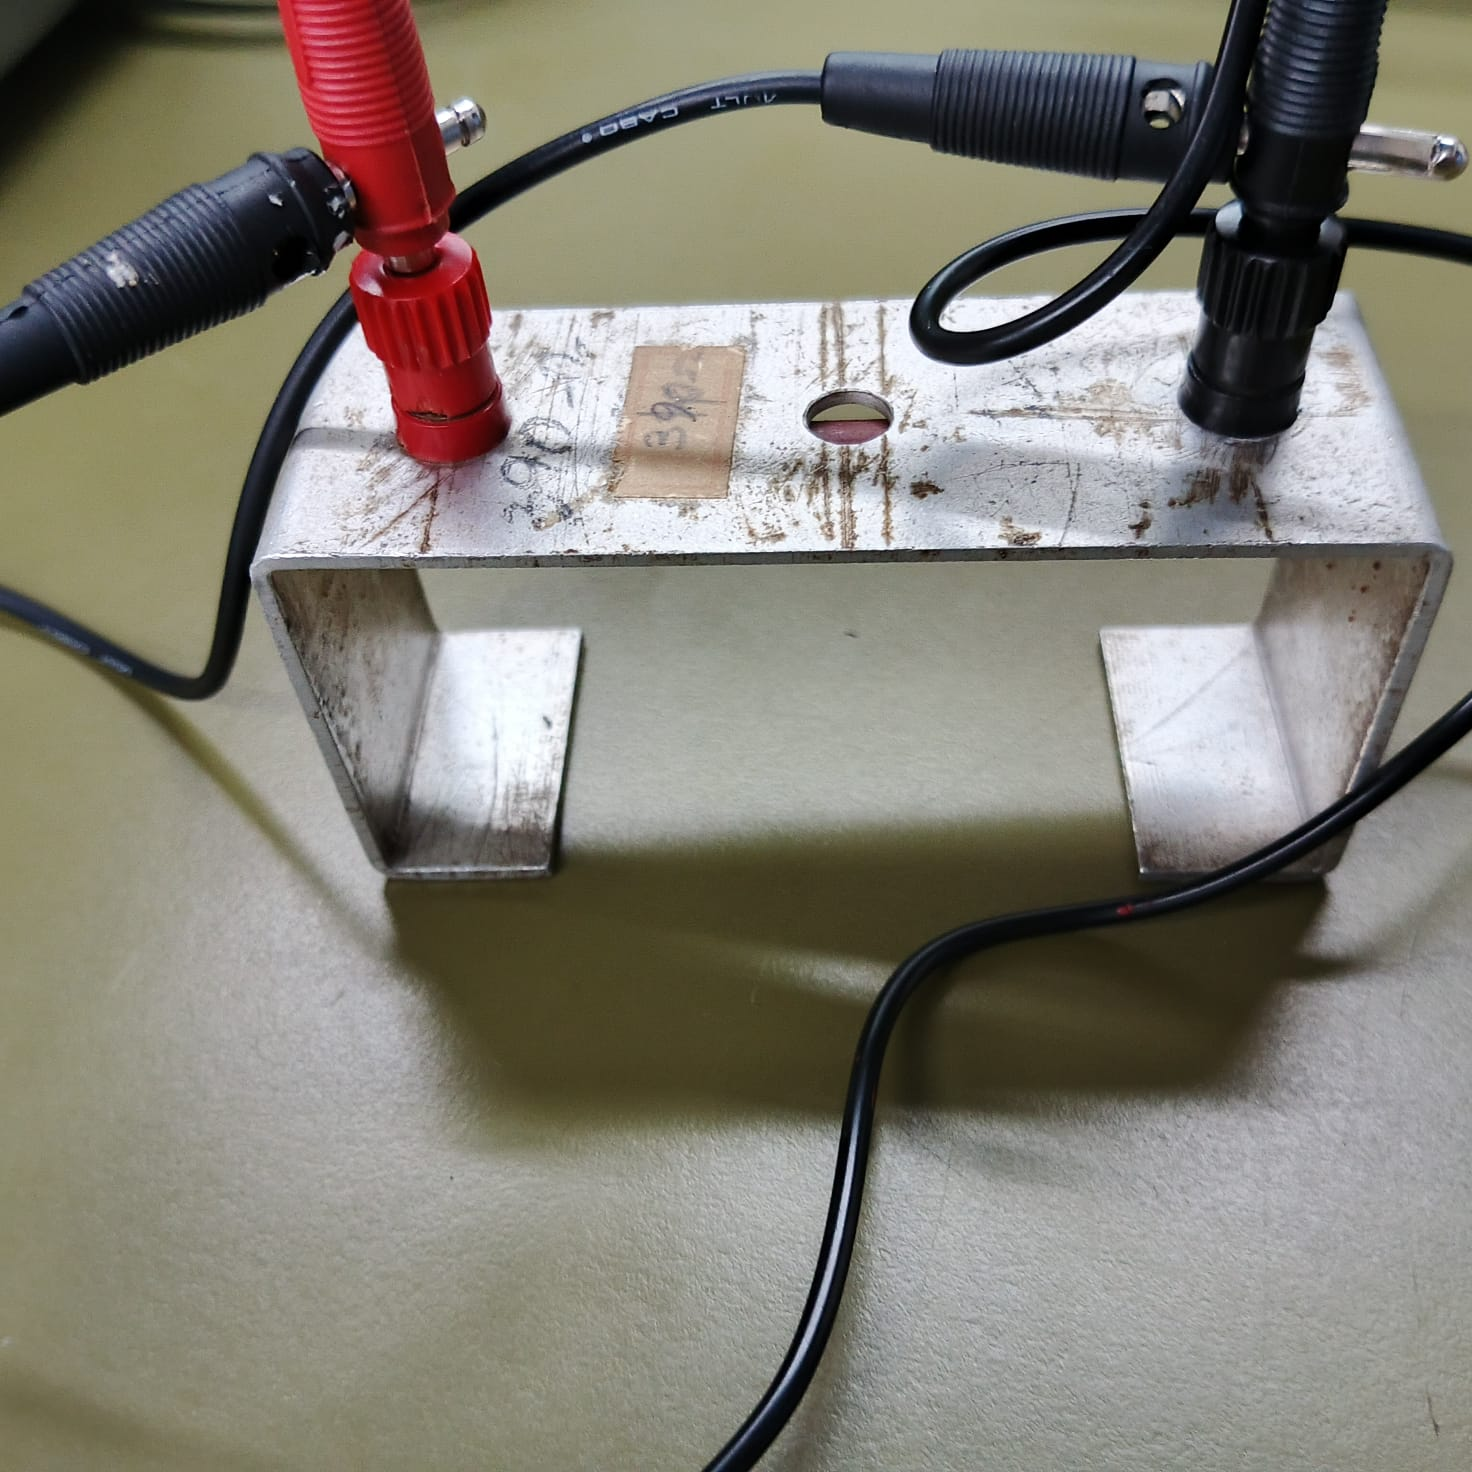
\includegraphics[width=0.4\linewidth]{./Figs/resistor.jpeg}
    \end{figure}
    
    \item Multímetro digital. \par\vspace{0.5\baselineskip}
                \begin{figure}[H]
      \centering
      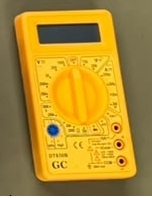
\includegraphics[width=0.4\linewidth]{./Figs/digital.jpg}
    \end{figure}
      
    \end{enumerate}

\subsection{Procedimento experimental}

Inicialmente, a fonte de alimentação foi conectada à rede elétrica e ligada, mantendo-se seus controles de tensão e corrente em condições adequadas para a realização das medições. Em seguida, o seletor de ajuste da fonte foi posicionado sucessivamente nas marcações 2, 4, 6, 8 e 10.

Para cada uma dessas posições, foram medidos os valores da diferença de potencial e da corrente elétrica fornecidos pela fonte. As medições de tensão foram realizadas com o voltímetro conectado em paralelo aos terminais de saída da fonte, enquanto as medições de corrente foram efetuadas com o amperímetro conectado em série com o circuito.

Em cada posição do seletor foram realizadas quatro medições independentes de tensão e quatro medições independentes de corrente. Os valores obtidos foram registrados em uma tabela, permitindo avaliar a repetibilidade das medições e as possíveis variações associadas aos instrumentos e à fonte de alimentação.

Para cada conjunto de quatro medições, calculou-se a média aritmética, dada por

\begin{equation}
\overline{x}
=
\frac{1}{n}
\sum_{i=1}^{n} x_i,
\label{eq:media_medidas}
\end{equation}

em que $x_i$ representa cada valor medido e $n=4$ corresponde ao número de medições realizadas em cada posição.

O desvio padrão amostral foi calculado por

\begin{equation}
s
=
\sqrt{
\frac{
\displaystyle\sum_{i=1}^{n}
\left(x_i-\overline{x}\right)^2
}{n-1}
},
\label{eq:desvio_padrao_medidas}
\end{equation}

em que $s$ representa o desvio padrão das medições. Esse parâmetro foi utilizado para avaliar a dispersão dos valores em torno da média e, consequentemente, a estabilidade das leituras obtidas em cada posição da fonte. As expressões da média aritmética e do desvio padrão amostral seguem as definições usuais para uma amostra de medições \parencite[seção 7.2.2]{nist2002}.

Ao final, os resultados de tensão e corrente foram apresentados na forma

\[
\overline{x} \pm s,
\]

para cada uma das posições analisadas.

\section{Resultados e Discussões}

Os valores medidos e os respectivos valores médios e desvios padrão amostrais são apresentados nas tabelas a seguir.

\begin{table}[H]
    \centering
    \caption{Valores de tensão e corrente observados nas diferentes posições da fonte.}
    \medskip
    \label{tab:medicoes}

    \begin{tabular}{
        c
        S[table-format=2.1]
        S[table-format=2.1]
    }
        \toprule
        \textbf{Posição}
        & {\textbf{Tensão} (\si{\volt})}
        & {\textbf{Corrente} (\si{\milli\ampere})} \\
        \midrule

        \multirow{4}{*}{2}
        & 4,5 & 3,5 \\
        & 5,0 & 3,6 \\
        & 5,2 & 4,0 \\
        & 4,5 & 2,7 \\
        \midrule

        \multirow{4}{*}{4}
        & 10,4 & 4,0 \\
        & 10,7  & 4,2 \\
        & 10,5  & 4,5\\
        & 9,8   & 3,4\\
        \midrule

        \multirow{4}{*}{6}
        & 16,0  & 5,0\\
        & 16,8  & 4,9\\
        & 16,0  & 4,8\\
        & 15,0  & 4,0\\
        \midrule

        \multirow{4}{*}{8}
        & 21,5  & 5,0\\
        & 21,0  & 5,2\\
        & 20,7  & 5,6\\
        & 21,0  & 5,3\\
        \midrule

        \multirow{4}{*}{10}
        & 26,5  & 5,0\\
        & 26,0  & 5,8\\
        & 26,0  & 5,8\\
        & 26,1  & 5,8\\
        \bottomrule
    \end{tabular}
\end{table}

Os valores médios e os respectivos desvios padrão amostrais estão
apresentados na Tabela~\ref{tab:estatisticas}.

\begin{table}[H]
    \centering
    \caption{Médias e desvios padrão amostrais da tensão e da corrente.}
    \label{tab:estatisticas}
    \medskip

    \begin{tabular}{
        c
        S[table-format=2.2]
        S[table-format=1.2]
        S[table-format=1.2]
        S[table-format=1.2]
    }
        \toprule
        {\textbf{Posição}}
        & {$\boldsymbol{\bar{V}}$ (\si{\volt})}
        & {$\boldsymbol{s_V}$ (\si{\volt})}
        & {$\boldsymbol{\bar{I}}$ (\si{\milli\ampere})}
        & {$\boldsymbol{s_I}$ (\si{\milli\ampere})} \\
        \midrule
        2  & 4.80  & 0.36 & 3.45 & 0.54 \\
        4  & 10.35 & 0.39 & 4.03 & 0.46 \\
        6  & 15.95 & 0.74 & 4.68 & 0.46 \\
        8  & 21.05 & 0.33 & 5.28 & 0.25 \\
        10 & 26.15 & 0.24 & 5.60 & 0.40 \\
        \bottomrule
    \end{tabular}
\end{table}

\section{Discussão dos resultados}

A Figura~\ref{fig:regressao} apresenta os cinco pontos formados pelos valores médios de tensão e corrente, juntamente com a reta de regressão linear.

\begin{figure}[H]
      \centering
      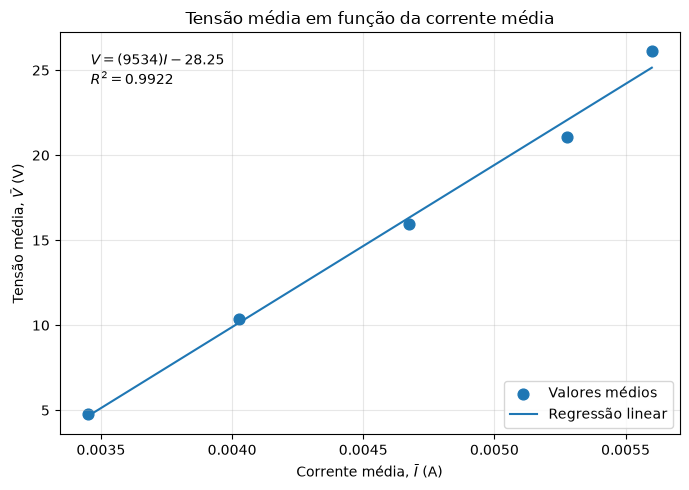
\includegraphics[width=0.8\linewidth]{./Figs/regressao_linear.png}
      \caption{Tensão média em função da corrente média e reta de regressão linear.}
      \label{fig:regressao}
\end{figure}

\subsection{Determinação gráfica da resistência elétrica} 

A resistência elétrica foi determinada pelo coeficiente angular da reta obtida no gráfico da tensão média em função da corrente média, conforme a relação $V=RI$. O ajuste foi realizado por regressão linear pelo método dos mínimos quadrados \parencite[seção 9.4]{ling2016}; o método dos mínimos quadrados é descrito por \textcite[seção 4.1.4.1]{nist2002}.

As leituras experimentais foram preservadas. O fator de escala do miliamperímetro foi determinado a partir da faixa utilizada no instrumento, sem empregar o valor nominal ou a medição direta do resistor para corrigir os dados.

\subsection{Fator de escala do miliamperímetro}

O mostrador do miliamperímetro apresenta uma escala de 0 a 75.
Considerando a utilização da faixa de 75 mA, o fator de escala é:

\[
f_{\mathrm{escala}}
=
\frac{75\ \mathrm{mA}}{75}
=
1\ \mathrm{mA/divisão}.
\]

Portanto, cada unidade indicada na escala corresponde a 1 mA.

O fator de escala do miliamperímetro foi determinado pela razão entre
a faixa de 75 mA e a escala de 0 a 75, resultando em 1 mA por divisão.
Assim, nenhuma alteração numérica foi aplicada às leituras médias.

A regressão linear dos cinco pares de valores médios forneceu uma resistência de aproximadamente \SI{9,53}{\kilo\ohm}, muito superior ao valor de \SI{390}{\ohm} obtido pela medição direta.

Além disso, o intercepto da reta foi significativamente diferente de zero. A comparação entre as correntes registradas e as correntes esperadas para um resistor de \SI{390}{\ohm} mostrou que não existe um único fator multiplicativo capaz de compatibilizar todos os pontos.

Dessa forma, a divergência não pode ser atribuída apenas à conversão
da escala do miliamperímetro. Os resultados indicam a possibilidade de
erro instrumental, ligação inadequada, defeito de calibração ou outro
problema ocorrido durante a aquisição das correntes.

\section{Conclusão}

Embora os valores médios tenham apresentado forte associação linear, a resistência obtida pelo coeficiente angular da regressão não foi compatível com a medição direta do resistor. A análise das leituras individuais mostrou que a discrepância não pode ser corrigida por um único fator de escala, indicando provável erro instrumental ou experimental durante a aquisição das correntes. 

\clearpage
\printbibliography[
  heading=bibintoc,
  title={Referências}
]

\newpage
\section{Anexos}

\subsection{Registro dos dados}

\begin{figure}[H]
      \centering
      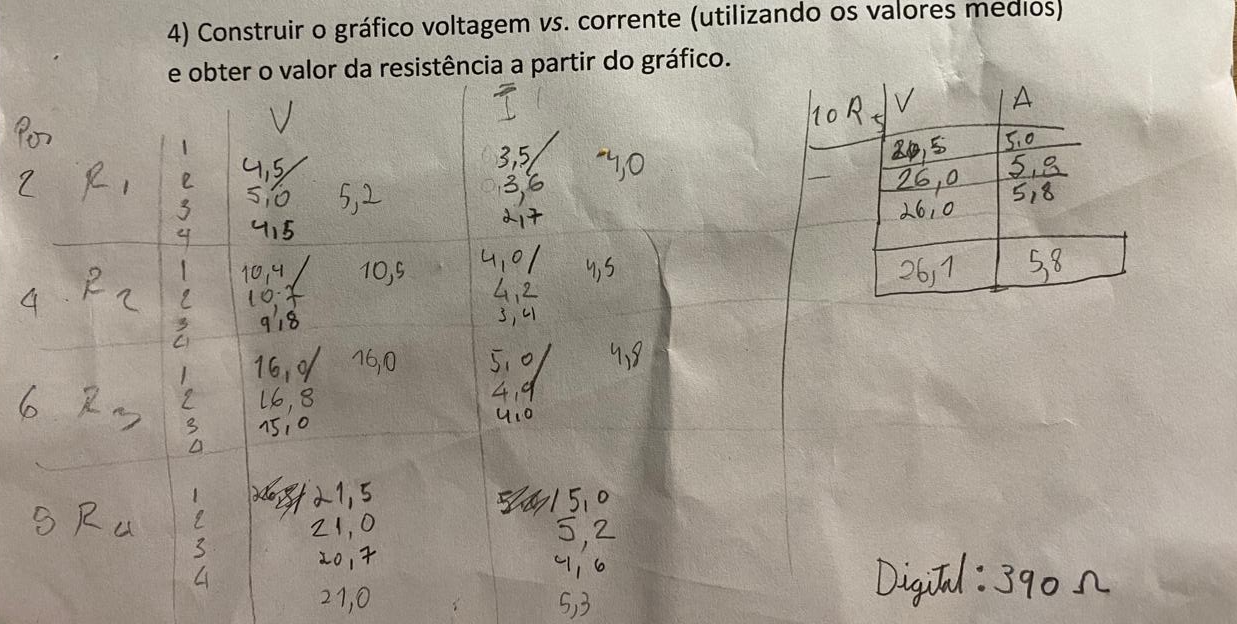
\includegraphics[width=\linewidth]{./Figs/registros.png}
      \caption{Registros manuscritos dos dados}
\end{figure}

\clearpage
\appendix

\includepdf[
    pages=-,
    addtotoc={
        1,
        section,
        1,
        {Notebook utilizado na análise dos dados},
        ap:notebook
    },
    pagecommand={\thispagestyle{plain}},
    scale=0.95
]{Apendices/lei_de_ohm_notebook.pdf}

\end{document}